\documentclass[../Hovedrapport.tex]{subfiles}
\begin{document}
%-----------------------------------------------------------------------
\chapter{Komponenter og energibalancer}
    \label{chap:dimensionering}
    \vspace{-30pt}
I dette kapitel vil kontrolflader, energibalancer og dertilhørende figurer blive opstillet for det overordnede system samt for systemets enkelte komponenter. Efterfølgende vil energibalancerne blive anvendt til at bestemme ydelseskravene til køleanlæggets komponenter. 
%-----------------------------------------------------------------------
\section{Energibalancer og kontrolflader (Alle)}
Når køleanlægget skal dimensioneres, skal kontrolflader og energibalancer bestemmes.
De stationære systemer tager udgangspunkt i nedenstående energibalance \citep{termo}:
\begin{align}
    \Sigma \dot{E}_{ind} + \Sigma \dot{E}_{gen} - \Sigma \dot{E}_{ud} = 0
\end{align}
For de ikke stationære systemer ser det ud som følger \citep{termo}:
\begin{align}
    \Sigma \dot{E}_{ind} + \Sigma \dot{E}_{gen} - \Sigma \dot{E}_{ud} = m \cdot c_p \cdot \dfrac{\Delta t}{\Delta \tau}
\end{align}
Kontrolfladerne afgrænser systemet, mens energibalancerne fortæller, hvilken energi de forskellige komponenter i systemet tilføres og afgiver ved krydsning af kontrolfladerne. Der vil i følgende underafsnit blive opstillet kontrolflader og energibalancer for kompressoren, fordamperen, kondensatoren og ventilen. Disse vil senere i rapporten blive brugt til at finde interessante værdier på komponenterne i systemet. I nedenstående figur fremgår kontrolfladernes placering med nummerering i systemet.

\begin{figure}[H] % (alternativt [H])
	\centering
	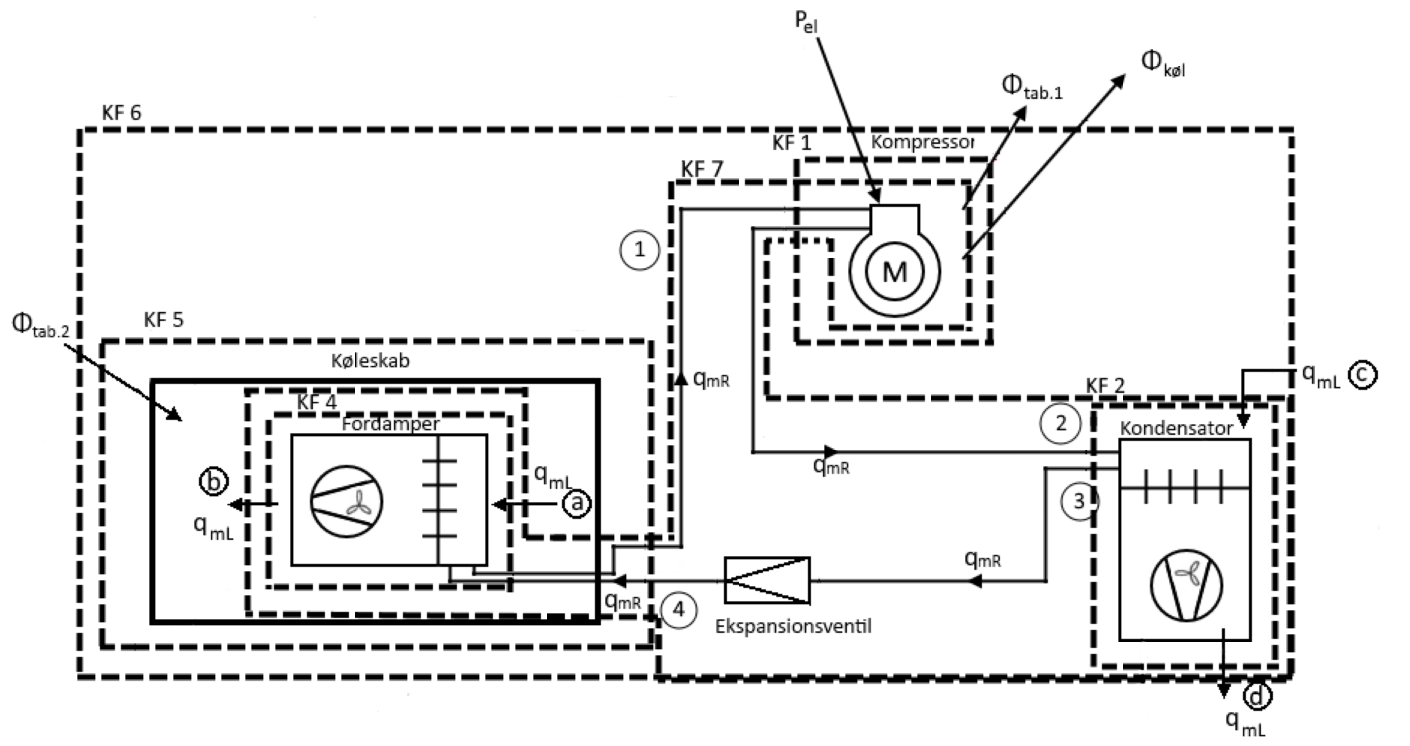
\includegraphics[width=1\textwidth]{Billeder/tingudennavn.png}
	\caption{\textit{Oversigt over køleanlægget}.}
	\label{fig:Anlægsoversigt}
\end{figure}
%----------------------------------------------------------------
\subsection{Kompressor (KF1)}
% Venstre søjle
\begin{minipage}[t]{0.5\textwidth}
Kompressoren modtager en elektrisk effekt, hvormed den komprimerer kølemidlet. Dette medfører, at gassens energiniveau stiger. Under denne kompression vil der være et varmetab i og med, at kompressionen ikke forløber med en isentropisk virkningsgrad på 1. Dog antages kompressionen at være adiabatisk \citep{termo}. Hertil antages kompressoren ligeledes at være luftkølet.
I figur \ref{fig:Kompressor_KF} fremgår kontrolflade 1, hvilket giver følgende energibalance:
\begin{align}
\label{eq:kompressorEB}
    P_{el}+q_{mR} \cdot (h_{1}-h_{2})-\Phi_{tab,1}-\Phi_{\textit{køl}} = 0
\end{align}
\end{minipage}
% Højre søjle:
\begin{minipage}[t]{0.5\textwidth}
\vspace{-30pt}
\begin{figure}[H]
\centering
	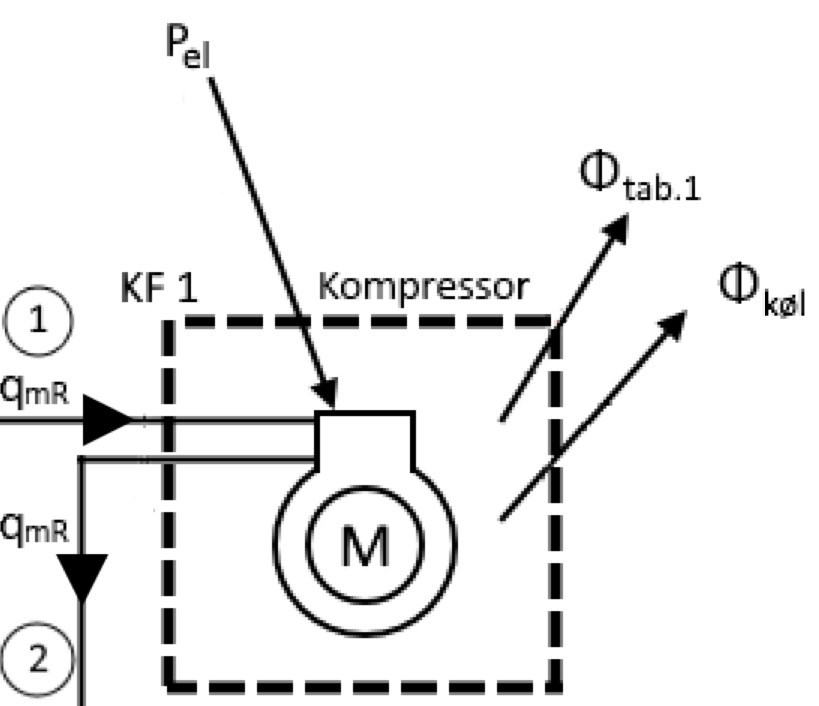
\includegraphics[width=0.8\textwidth]{Billeder/KF_1.png}
	\caption{\textit{Kontrolflade omkring kompressoren}.}
	\label{fig:Kompressor_KF}
\end{figure}
\end{minipage}
%-----------------------------------------------------------------------------
\subsection{Kondensator (KF2)}
% Venstre søjle
\begin{minipage}[t]{0.5\textwidth}
Kondensatoren har til opgave at afgive varme fra det overhedede kølemiddel til omgivelserne. Igennem kondensatoren er trykket konstant, men der sker en faseovergang fra gas- til væskeform, da energiniveauet falder.
I figur \ref{fig:Kondensator-KF} fremgår kontrolflade 2. Denne kontrolflade er dog opdelt i to, så der er en for henholdsvis kølemidlet (rød) og for luften (blå). Dette giver følgende energibalancer:
\begin{align}
\label{eq:kondensatorEB}
    q_{mR} \cdot (h_{2} - h_3) - \Phi_{k} = 0   &&&\text{Kølemiddelside} \\
    q_{mL,k} \cdot (h_{c}-h_{d}) + \Phi_{k} = 0       &&& \text{Luftside}
\end{align}
\end{minipage}
% Højre søjle:
\begin{minipage}[t]{0.5\textwidth}
\vspace{-30pt}
\begin{figure}[H]
\centering
	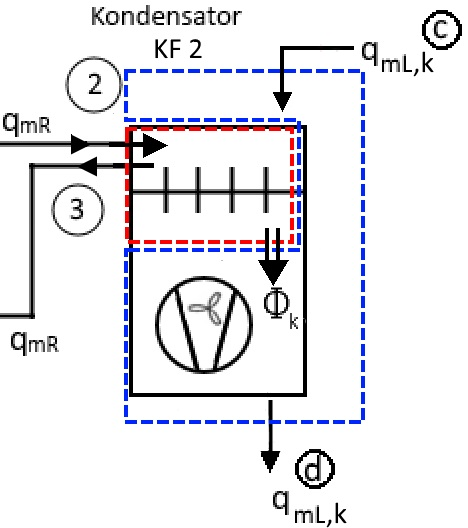
\includegraphics[width=0.8\textwidth]{Billeder/KF_2}
	\caption{\textit{Kondensator med kontrolflade}.}
	\label{fig:Kondensator-KF}
\end{figure}
\end{minipage}
\subsection{Ekspansionsventil (KF3)}
% Venstre søjle
\begin{minipage}[t]{0.5\textwidth}
Ventilens formål er at sænke trykket fra kondensatoren til fordamperen. Denne proces foregår, ligesom ved kompressoren, adiabatisk. 
I figur \ref{fig:Ekspansionsventil-KF} fremgår kontrolflade 3, hvilket giver nedenstående energibalance, idet $h_3$ og $h_4$ er lig med hinanden:
\begin{align}
    q_{mR} \cdot(h_{3}-h_{4})=0  
\end{align}
\end{minipage}
% Højre søjle:
\begin{minipage}[t]{0.5\textwidth}
\vspace{-40pt}
% Figur:
\begin{figure}[H] % (alternativt [H])
	\centering
	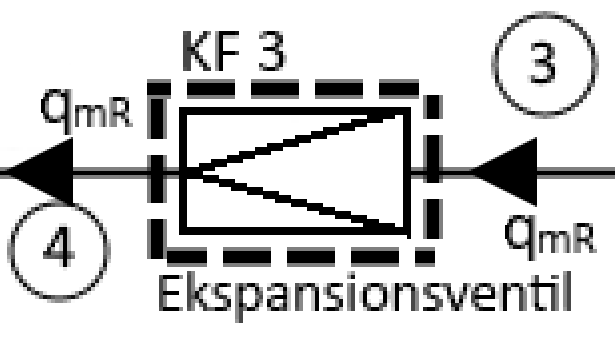
\includegraphics[width=0.7\textwidth]{Billeder/KF_3.png}
	\caption{\textit{Ekspansionsventil med kontrolflade}.}
	\label{fig:Ekspansionsventil-KF}
\end{figure}
\end{minipage}
%-----------------------------------------------------------------------
\subsection{Fordamper (KF4)}
% Venstre søjle
\begin{minipage}[t]{0.5\textwidth}
I fordamperen optages varmen fra den omkringliggende luft. Denne varmestrøm kaldes kuldeydelsen og betegnes $\Phi_0$. Varmen, som fordamperen optager, får kølemidlet til at fordampe ved konstant tryk og temperatur, hvorefter det bliver ført videre til kompressoren.
I figur \ref{fig:Fordamper-KF} fremgår kontrolflade 4. Denne er ligesom for kondensatoren også delt op i to, hvilket giver følgende energibalancer: 
\begin{align}
\label{eq:fordamperkm}
q_{mR} \cdot (h_4-h_1) + \Phi_0 = 0     &&&\text{Kølemiddelside} \\
q_{mL,f} \cdot (h_{a}-h_{b}) - \Phi_0 = 0     &&&\text{Luftside}
\end{align}
\end{minipage}
% Højre søjle:
\begin{minipage}[t]{0.5\textwidth}
%\vspace{-40pt}
% Figur:
\begin{figure}[H] % (alternativt [H])
	\centering
	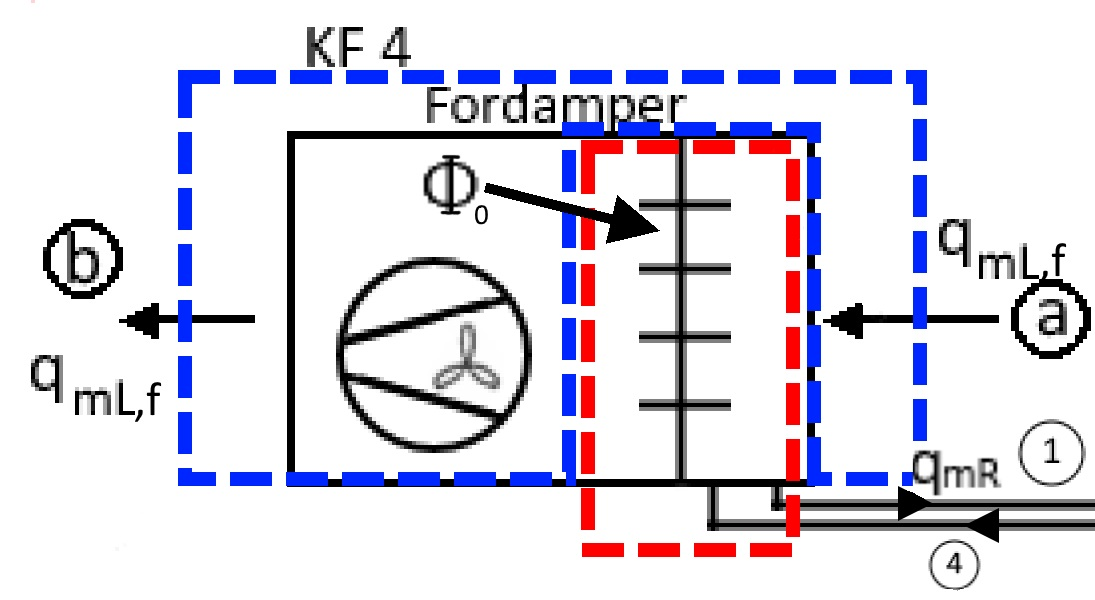
\includegraphics[width=1\textwidth]{Billeder/KF_4}
	\caption{\textit{Fordamper med kontrolflader}.}
	\label{fig:Fordamper-KF}
\end{figure}
\end{minipage}
%-----------------------------------------------------------------------
\subsection{Køleskabet (KF5)}
% Venstre søjle
\begin{minipage}[t]{0.5\textwidth}
I køleskabet sker selve nedkølingen af diverse indsatte emner, med individuelle masser og specifikke varmekapaciteter, ved hjælp af fordamperen. Ved en nedkøling er der ikke tale om et stationært system, og på baggrund af dette bliver energibalancen dermed:
\begin{align}
\label{eq:Skab}
q_{mR} \cdot (h_4-h_1) + \Phi_{tab,2} =  {m \cdot c_p \cdot \dfrac{\Delta t}{\Delta \tau}}
\end{align}
$\Phi_{tab,2}$ betegner varmestrømmen fra luften omkring køleskabet og ind i dette som følge af temperaturdifferensen. Når emnerne i køleskabet har samme temperatur som den omkringliggende luft, vil temperaturdifferensen være nul, hvorved højre side af 
\end{minipage}
% Højre søjle:
\begin{minipage}[t]{0.5\textwidth}
%\vspace{-40pt}
\begin{figure}[H] % (alternativt [H])
	\centering
	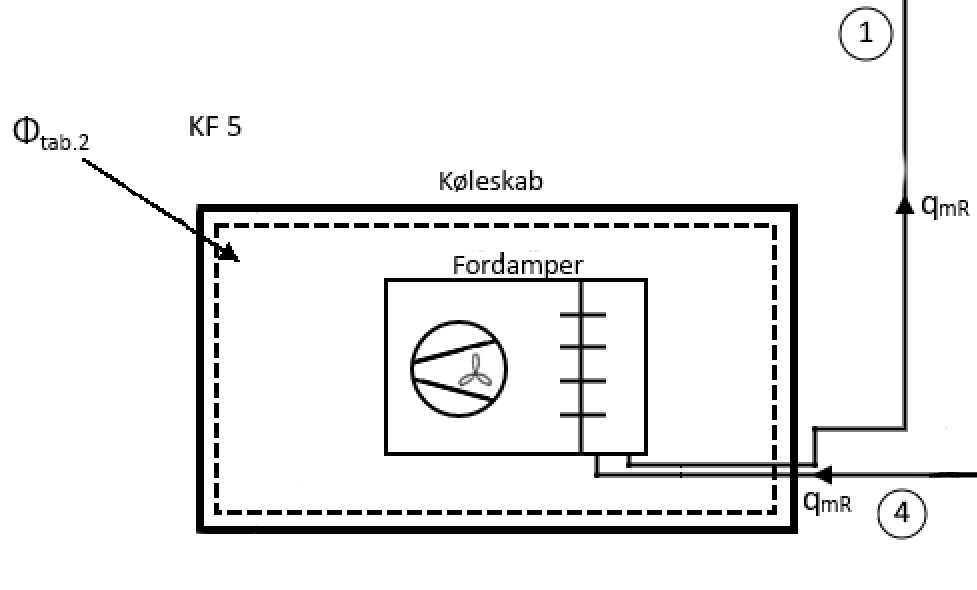
\includegraphics[width=1\textwidth]{Billeder/KF_5.png}
	\caption{\textit{Fordamper med kontrolflader}.}
	\label{fig:Skab-KF}
\end{figure}
\end{minipage}
ovenstående ligning også giver nul. Hermed giver energibalancen nul og systemet er således stationært:
\begin{align}
\label{eq:Skab}
q_{mR} \cdot (h_4-h_1) + \Phi_{tab,2} = 0
\end{align}
%-----------------------------------------------------------------------
\subsection{Hele systemet (KF6)}
Energibalancen som følge af kontrolfladen omkring hele systemet kan være enten stationær eller ikke-stationær. Ved sidstnævnte tilfælde vil energibalancen være som følger:
\begin{align}
\label{eq:helesystemEB}
    P_{el} - \Phi_{tab,1} - \Phi_{\textit{køl}} + \Phi_{tab,2} - q_\text{mL,k}\cdot (h_c - h_d) = m \cdot c_p \cdot \dfrac{\Delta t}{\Delta \tau}
\end{align}
% Figur:
\begin{figure}[H] % (alternativt [H])
	\centering
	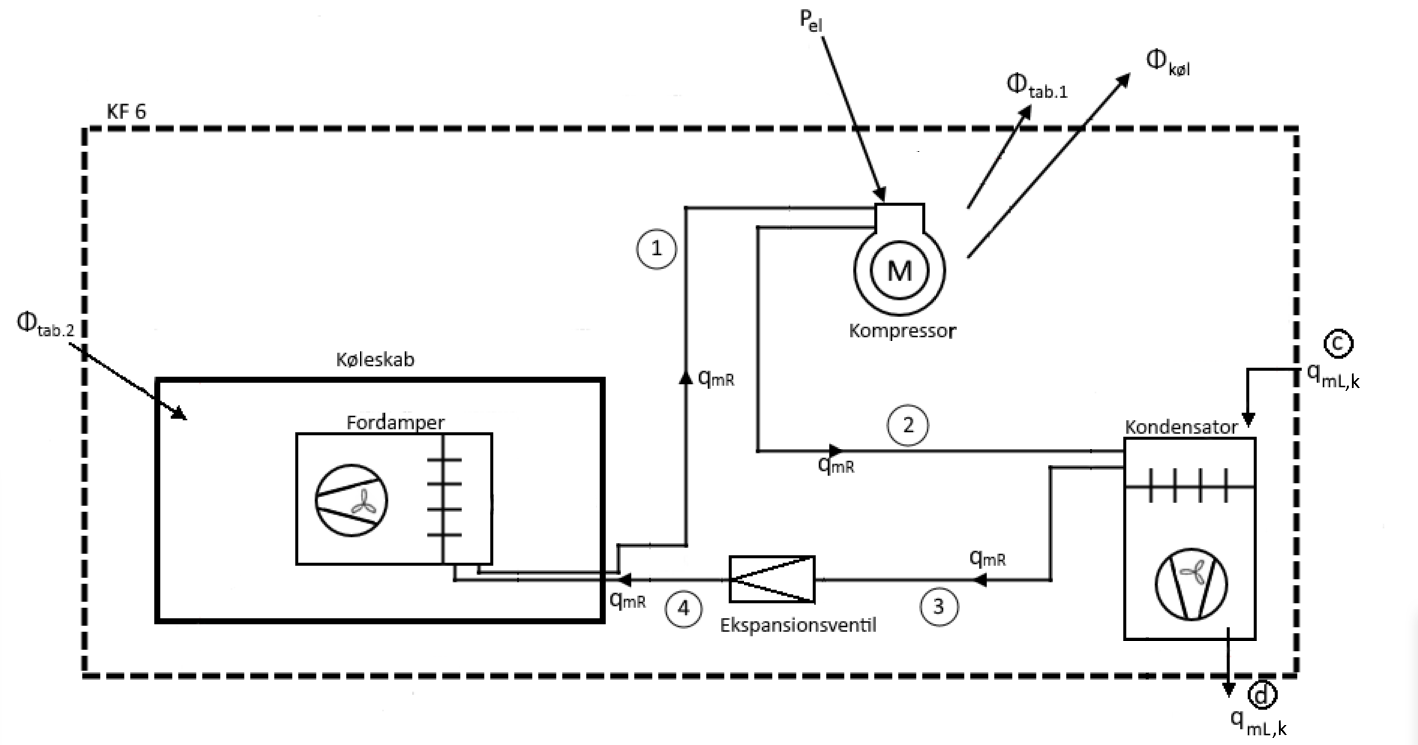
\includegraphics[width=1\textwidth]{Billeder/KF_6.png}
	\caption{\textit{Hele systemet med kontrolflade}.}
	\label{fig:Hele systemet-KF}
\end{figure}
%-----------------------------------------------------------------------
\subsection{Køleanlægget (KF7)}
Den sidste kontrolflade er om hele køleanlægget (se figur \ref{fig:kun_sys}). Her kigges der på energistrømme der kommer udefra og strømmer indover anlæggets kontrolflade. I dette tilfælde er de primære massestrømme ved varmevekslerne, hvilket vil sige de massestrømme, der bliver blæst over fordamperen og kondensatoren i form af luft. Foruden dette, bliver der også tilført en elektrisk effekt $\text{P}_\text{el}$, og systemet mister energi i form af et kølingstab $\Phi_\text{køl}$ og et tab i kompressoren $\Phi_{tab,1}$. Det skal bemærkes, at de to luftmassestrømme over kondensatoren og fordamperen i ligning \ref{eq:helesystemEB2} benævnes henholdsvis $\Phi_k$ og $\Phi_0$.
\begin{align}
\label{eq:helesystemEB}
&P_{el} +q_{mL,f} \cdot (h_a - h_b) - \Phi_{\textit{køl}} - \Phi_{tab,1} + q_{mL,k} \cdot (h_c - h_d) = 0 \\
\label{eq:helesystemEB2}
&P_{el} +\Phi_0 - \Phi_{\textit{køl}} - \Phi_{tab,1} - \Phi_k = 0
\end{align}
% Figur:
\begin{figure}[H] % (alternativt [H])
	\centering
	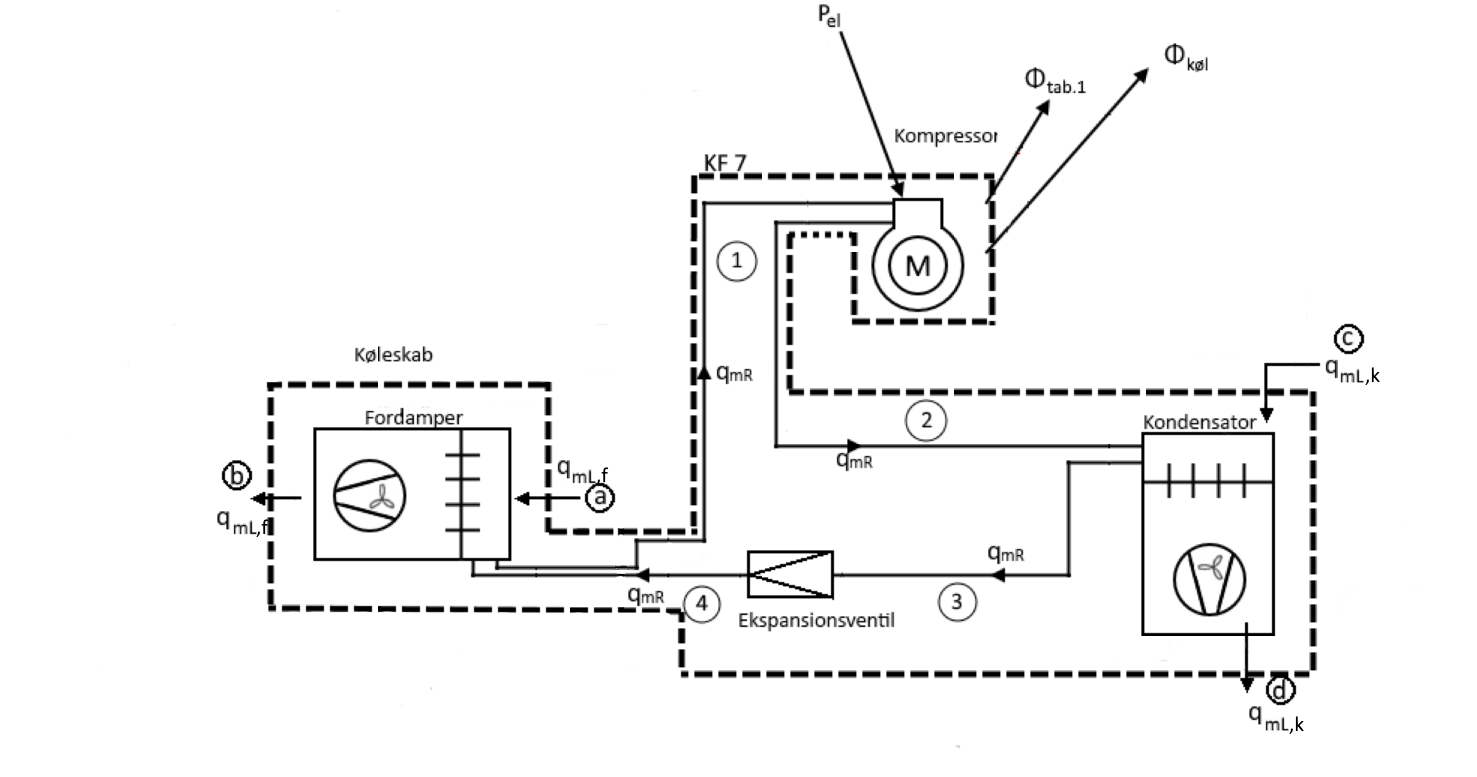
\includegraphics[width=1\textwidth]{Billeder/KF_7.png}
	\caption{\textit{Kølesystemets kontrolflade}.}
	\label{fig:kun_sys}
\end{figure}

\section{Udvælgelse af kompressor (U.H. \& B.B.)}
    \label{sec:dim_kompressor}
I de følgende underafsnit udvælges en kompressor til anlægget. Dette beregnes på baggrund af den mængde varme, som flaskerne i køleskabet kan afgive, samt varmetabet gennem køleskabets vægge. 
%-----------------------------------------------------------------------
\subsection{Nøgletal}
    \label{sec:noegletal}
For at køleskabet kan være funktionsdygtigt under det beskrevne worst-case scenarie i problemformuleringen, er det vigtigt, at det kan køle ned til den ønskede temperatur mellem \SI{3} og \SI{5}{\celsius}. I udvælgelsesfasen foretages beregningerne efter en ønsket temperatur på \SI{4}{\celsius} i køleskabet. Dette medfører, at kølemidlet, der strømmer gennem anlægget, skal have en lavere temperatur end den ønskede i køleskabet. Fordampningstemperaturen ønskes derfor til -\SI{8}{\celsius} med en overhedning på \SI{8}{\kelvin}.
% Nedentstående skal læses igennem igen.
Kondenseringstemperaturen for anlægget vælges på baggrund af, at denne temperatur erfaringsmæssigt sættes til at være 12 - 20 \si{\kelvin} højere end omgivelsestemperaturen \citep{koleteknik} tabel 11.14. Idet $\SI{30}{\celsius}$ er valgt som den maksimale omgivelsestemperatur om køleskabet vælges kondenseringstemperaturen til $\SI{50}{\celsius}$. Hertil vælges en underkøling på $\SI{5}{\kelvin}$.

Ydermere er det vigtigt, at varmevekslerne holdes rene, hvilket er med til at sikre en konstant luftstrøm over disse. Dette skyldes, at skidt og snavs vil øge den termiske modstand og samtidig fungere som en fysisk barriere for luftstrømmen.

En oversigt med nøgletal for systemet kan nu opstilles ud fra ovenstående temperaturer, tryk samt kølemiddelstypen og fremgår af nedenstående tabel \ref{tab:procesval}.
\begin{table}[H] 
\renewcommand{\arraystretch}{1.4}
\centering
\vspace{-0.3cm}
\begin{tabular}{|c|c|c|c|c|}  \cline{1-5} \rowcolor[gray]{0.7}
\multicolumn{5}{|c|}{\textbf{Anlægstemperaturer}}      \\ \hline \rowcolor[gray]{.8}
\textbf{Proces} & \textbf{T}    & \textbf{P}    & \textbf{$\rho$}   & \textbf{h} \\ \hline 

	\textbf{1}                           & \SI{0}{\celsius}             & \SI{2,17}{\bar}     & \SI{10,41}{\frac{kg}{m^3}}        & \SI{400,7}{\frac{kJ}{kg}}       \\  \hline
	\textbf{2s}                          & \SI{63,04}{\celsius}            & \SI{13,18}{\bar}    & \SI{60,17}{\frac{kg}{m^3}}        &  \SI{438,9}{\frac{kJ}{kg}}    \\\hline
	\textbf{3}                           & \SI{45}{\celsius}            & \SI{13,18}{\bar}    & \SI{1127}{\frac{kg}{m^3}}          & \SI{263,9}{\frac{kJ}{kg}}       \\ \hline
	\textbf{4}                           & \SI{-8}{\celsius}            & \SI{2,17}{\bar}     & \SI{10,41}{\frac{kg}{m^3}}          & \SI{263,9}{\frac{kJ}{kg}}       \\ \bottomrule
	\end{tabular} 
	\caption{\textit{Procesværdierne for køleskabet}.} 
	\label{tab:procesval} 
\end{table}
Log p,h diagrammet for anlægget er optegnet i afsnit \ref{sec:logphdiagram}, når de forskellige entalpier i tilstand 2 er bestemt.
%-----------------------------------------------------------------------
\subsection{Størrelse af kompressor (U.H. \& B.B.)}
    \label{sec:stoerrelse_kompressor}
 Kompressoren størrelse bliver nu bestemt. Dette gøres ved en overslagsberegning på, hvor meget varme plastikflasker, af typen PET, kan afgive pr. tidsenhed. Da dette er en indledende overslagsberegning, ses der bort fra varmestrømmen til nedkølingen af den eksisterende luft i køleskabet, samt  varmetab ved åbning af køleskabets dør. Denne indledende overslagsberegning tager udgangspunkt i formlen for varmetransmission, som ser ud som følger \citep{termo}: 
\begin{align}
    \label{eq:varmestrøm}
    \Phi=U \cdot A \cdot (t_{ind}-t_{ud})
\end{align} % Ulrik har ændret i temperaturerne. Lad venligst vær med at ændre dem tilbage.
Her antages det, at 40 flasker skal nedkøles fra en temperatur på $t_{ud}=\SI{21}{\celsius}$ til $t_{ind} = \SI{4}{\celsius}$. I disse beregninger antages det, at flaskerne er cylinderformede med et ydre overfladeareal pr. flaske på  $A_{u,flaske} = \SI{285}{cm^2}$. En illustration af flaskens dimensioner og beregningen af overfladearealet fremgår af appendiks \ref{sec:apndx_flaskedim}. 

Nu bestemmes varmegennemgangstallet med henblik på at skulle indsættes i ligning \ref{eq:varmestrøm}. $U_u$ bestemmes ud fra nedenstående ligning \citep{termo}:
\begin{align}
    \label{eq:varmegennemgangstal}
    U_u=\dfrac{1}{\dfrac{1}{\alpha_i}\cdot \dfrac{d_u}{d_i}+\dfrac{d_u}{2\cdot \lambda}\text{ln}\left(\dfrac{d_u}{d_i} \right)+\dfrac{1}{\alpha_u}}
\end{align}
I og med dette stadig er en overslagsberegning bestemmes varmeovergangstallet indvendigt og udvendigt ud fra erfaringstal fra bilag \ref{sec:bil_erfaringstal_U}. Indvendigt i flasken er der fri strømning af vand og dermed antages $\alpha_i=\SI{100}{\frac{W}{m^2 \cdot K}}$. Udvendigt på flasken er der en tvungen strømning af luft, hvilket erfaringsmæssigt ligger i intervallet 10 til $\SI{100}{\frac{W}{m^2 \cdot K}}$. Ud fra dette antages $\alpha_u=20\si{\frac{W}{m^2 \cdot K}}$. Udover de erfaringsmæssigt bestemte varmeovergangstal skal der i ligning \ref{eq:varmegennemgangstal} også bestemmes en varmekonduktivitet for plasttypen PET, hvilket findes via programmet \textit{Edupack} til $\lambda=0,15\si{\frac{W}{m \cdot K}}$. Når tallene indsættes i ligningen udregnes den udvendige U-værdi til følgende:
\begin{align}
    U_u=\dfrac{1}{\dfrac{1}{\alpha_i}\cdot \dfrac{d_u}{d_i}+\dfrac{d_u}{2\cdot \lambda_{PET}}\text{ln}\left(\dfrac{d_u}{d_i} \right)+\dfrac{1}{\alpha_u}}=\SI{15,92}{\frac{W}{m^2 \cdot K}}
\end{align}
Herpå kan varmestrømmen for en flaske findes ved ligning \ref{eq:varmestrøm}.
\begin{align}
    \Phi_{flaske}=U_u \cdot A_u \cdot (t_{ud}-t_{ind})=7,65 \si{\watt}
\end{align}
For at få den samlede varmestrøm for alle flaskerne multipliceres antallet af flasker, \textit{N}, med $\Phi_{flaske}$.
\begin{align}
    \label{eq:flaske_samlet}
    \Phi_{f,sam}=\Phi_{flaske}\cdot N=306 \si{\watt}
\end{align}
Dette er vel at mærke kun så længe temperaturintervallet er uændret. Jo mindre temperaturforskellen mellem køleskabsluften og vandet i vandflasken bliver, desto mindre bliver varmestrømmen. Kompressoren udvælges dog for den største temperaturforskel, da dette giver den største varmestrøm, og dermed den største belastning på kompressoren gennem fordamperen.
%-----------------------------------------------------------------------
\subsubsection*{Tab gennem væggen}
Gennem væggene på køleskabet vil der ske en varmestrøm fra den omkringliggende luft til den køligere luft inde i køleskabet. Varmestrømmen sker ved konduktion gennem køleskabets vægge. Der vil i det følgende blive beregnet et overslag for, hvor stor denne varmestrøm vil være ved en driftsituation med \SI{4}{\celsius} inde i køleskabet og \SI{30}{\celsius} udenfor.

Konstanter, som benyttes til beregning af varmestrøm gennem væggene, fremgår af nedenstående tabel:
\renewcommand{\arraystretch}{1.3}
\begin{table}[H]
\centering
\begin{tabular}{|c|c|c|} \hline \rowcolor[gray]{0.7} 
\multicolumn{3}{|c|}{\textbf{Konstanter til beregning}} \\ \hline \rowcolor[gray]{0.8}
\textbf{Betegnelse} & \textbf{Beskrivelse} & \textbf{Værdi} \\ \hline
$t_\text{Lu}$       & Lufttemperatur uden for køleskab                                      & \SI{30}{\celsius} \\ \hline
$t_\text{Li}$       & Lufttemperatur inde i køleskab                                        & \SI{4}{\celsius} \\ \hline
$t_\text{væg}$      & Vægtykkelse                                                           & \SI{5}{cm} \\ \hline
$b_\text{ud}$       & Udvendig bredde                                                       & \SI{60}{cm} \\ \hline

$H_\text{ud}$       & Udvendig højde                                                        & \SI{119}{cm} \\ \hline
$\alpha_\text{ud}$   & Ydre varmeovergangstal (overslag - fri strømning luft)            & \SI{5}{\frac{W}{m^2\cdot K}} \\\hline
$\alpha_\text{ind}$  & Indre varmeovergangstal (overslag - tvungen strømning luft)       & \SI{20}{\frac{W}{m^2\cdot K}} \\\hline
$\lambda_{PS,skum}$ & Varmekonduktivitet for opskummet polystyren                                               & \SI{0,03}{\frac{W}{m\cdot K}} \\\hline
\end{tabular}
\caption{\textit{Konstanter til beregning varmetab igennem vægge og kuldeydelse}.}
\vspace{-10pt}
\end{table}
Varmestrømmen gennem væggene vil blive regnet ud fra det varmevekslende areal der i dette tilfælde betragtes som det udvendige areal. Dette udregnes på samme måde som i formel \ref{eq:varmestrøm}. Det udvendige areal består af køleskabets bund og top samt de fire sider:
\begin{equation}
    A_\text{skab} = 2\left({b_\text{ud}}^2 \right) + 4(b_\text{ud}\cdot H_\text{ud}) = \SI{3,58}{m^2}
\end{equation}
Varmegennemgangstallet, $U_{u,skab}$, beregnes:
\begin{equation}
    U_{u,skab} = \left( \frac{1}{\alpha_\text{ud}} + \frac{t_\text{væg}}{\lambda_\text{PS,skum}} + \frac{1}{\alpha_\text{ind}} \right)^{-1} = \SI{0,522}{\frac{W}{m^2\cdot K}}
\end{equation}
Ud fra ovenstående kan varmestrømmen gennem væggene nu bestemmes til:
\begin{equation}
    \label{eq:varmestroem_gennem_vaeg}
    \Phi_\text{tab} = U_{u,skab} \cdot A_\text{skab} \cdot \left( t_\text{Lu} - t_\text{Li} \right) = \SI{48,56}{W}
\end{equation}
Varmestrømmene fra flaskerne ligning \ref{eq:flaske_samlet} og de ydre omgivelser lægges nu sammen, hvorved den samlede varmestrøm findes ved følgende:
\begin{align}
    \label{eq:samletvarmestroemfraudregninger}
    \Phi_{0,behov}=\Phi_{tab}+\Phi_{f,sam}=\SI{354,6}{\watt}
\end{align}

Herved er kuldeydelsen det kræves at kompressoren skal kunne levere beeregnet til at være $\SI{354,6}{\watt}$.
%-----------------------------------------------------------------------
\subsection{Kompressorspecifikationer}
% Indskrivning af nøgletal efter valg
\label{sec:kompspec}
Ud fra bestemte anlægstemperaturer i afsnit \ref{sec:noegletal} og de tidligere bestemte værdier i afsnit \ref{sec:stoerrelse_kompressor} udvælges kompressoren \textit{BD350GH 24V DC} fra Danfoss ved indtastning i softwaren \textit{Danfoss Coolselector}. Indtastningen i \textit{Coolselector} fremgår af bilag \ref{sec:bil_kompressor_coolpack}. Denne kompressor vurderes til at være tilstrækkelig stor på baggrund af de førbestemte værdier trods det, at den er $\SI{20,6}{\watt}$ for lille sammenlignet med overslagsberegningen i forrige afsnit. Denne forskel vil, hvis antagelserne er korrekte, medføre en kortvarig temperaturstigning i køleskabet, da kompressoren i situationen er en smule for lille.  Kompressorens vigtigste tekniske specifikationer fremgår af tabel \ref{tab:kompressor_Data}:
%------------------------------TABEL START for kompressor data----------------------------
\begin{table}[H] 
	\centering
	\begin{tabular}{|c|c|c|c|} \rowcolor[gray]{0.7} \hline
	\multicolumn{4}{|c|}{\textbf{Kompressordata}}      \\ \hline \rowcolor[gray]{.8} \hline
	\textbf{Betegnelse}       & \textbf{Værdi}            & \textbf{Forklaring}                               & \textbf{Kilde}        \\ \hline 
	
	\text{R134a}            &                           & Kølemiddel                                        & Ønsket \\ \hline  
	\Phi_0                  & \SI{334}{\watt}           & Kuldeydelse                                        & Bilag \ref{sec:bil_kompressor_coolpack} \\ \hline  
	\Phi_k                  & \SI{530}{\watt}           & Varmeydelse                                        & Bilag \ref{sec:bil_kompressor_coolpack} \\ \hline   
	V_s           & \SI{5,08}{\cm^3}          & Slagvolumen                                       & Bilag \ref{sec:bil_kompressor_coolpack}              \\ \hline 
	RPM_\text{max}          & \SI{4000}{RPM}            & Max RPM af kompressor                             & Bilag \ref{sec:bil_kompressor_coolpack}              \\ \hline 
	RPM_\text{min}          & \SI{2500}{RPM}            & Min RPM af kompressor                             & Bilag \ref{sec:bil_kompressor_coolpack}              \\ \hline 
	\end{tabular} 
	\caption{\textit{Variabeloversigt, fra \citep{Coolselector} til dimensionering af fordamper}} 
	\label{tab:kompressor_Data} 
	\vspace{-20pt}
\end{table}
\newpage
Kuldeydelsen, som kompressoren kan sikre, ved forskellige omdrejningstal, fremgår af tabel \ref{tab:Kompressor_koleydelse_Data} 
\begin{table}[H] 
	\centering
	\begin{tabular}{|c|c|}  \cline{1-2} \rowcolor[gray]{0.7} \hline
	\multicolumn{2}{|c|}{\textbf{Kompressorens kuldeydelse}}      \\ \cline{1-2} \rowcolor[gray]{.8} \hline
	\textbf{  Omdrejningstal  }   & \textbf{  Kuldeydelse  }        \\ \cline{1-2}
	2500 RPM        & \SI{222}{\watt}                               \\ \cline{1-2} 
	3000 RPM        & \SI{267}{\watt}                               \\ \cline{1-2} 
	3500 RPM        & \SI{300}{\watt}                               \\ \cline{1-2} 
	4000 RPM        & \SI{334}{\watt}                               \\ \cline{1-2}
	\end{tabular} 
	\caption{\textit{Oversigt over kuldeydelse fra kompressor BD350GH 24 V.}} 
	\label{tab:Kompressor_koleydelse_Data} 
	\vspace{-20pt}
\end{table}
%-----------------------------------------------------------------------
\subsection*{Virkningsgrader} 
\label{sec:virkgrad}
% Note: Virkningsgraderne er opdateret den 10.12-2018
% ---- kommmentar ----
% Når det tales om virkningsgrader, så bør vi have virkningsgrader sat på i et skema med : 2500 - 4000 ved 35 degC og 2500 - 4000 rpm ved 50 degC. 
Kompressorens volumetriske og isentropiske virkningsgrad bestemmes i appendiks \ref{sec:apndx_kompressor_virkningsgrad}, hvor disse virkningsgrader er fundet til henholdsvis $\eta_{V}=0,69$ og $\eta_{s}=0,49$ ved et trykforhold på $6,07$, som er angivet i afsnit \ref{sec:noegletal}. Den volumetriske virkningsgrad er forholdet mellem kompressorens slagvolumenstrøm, $q_{V,s}$, og volumenenstrømmen, $q_{V1}$, som rent praktisk kan suges ind i kompressoren. Den isentropiske virkningsgrad for kompressoren er defineret som forholdet mellem den isentropiske effekt og den tilførte el-effekt \citep{termo}:
\begin{equation}
    \eta_{s,k}=\frac{P_{is}}{P_{el}}
\end{equation}
Disse værdier bliver senere brugt til at udarbejde et log p,h-diagram.
%----------------------------------------------------------------------
\end{document}
